\chapter{Evakuierung nach Rennersdorf und Befreiung in Görlitz}

Der Begriff des \glqq Todesmarsches\grqq~ist keine Wortschöpfung der Historiker, sondern von den Häftlingen der Konzentrationslager geprägt worden. Darunter verstehen sich erzwungene Märsche bewachter Gefangenenkolonnen über längere Distanzen und unter schlechten Bedingungen, in deren Verlauf viele der Häftlinge brutal gefoltert und ermordet wurden\footnote{Israel Gutman: Enzyclopädie des Holocaust, Band 3, S. 1412.}. Insbesondere in der Endphase des Krieges, als sich die alliierten Armeen den Lagern bedrohlich näherten, stellten viele Konzentrationslager ihre Funktion ein und \glqq evakuierten\grqq~die Gefangenen in andere Lager. Nicht um deren Leben willen, sondern um deren Arbeitskraft für die deutsche Kriegswirtschaft weiter ausbeuten zu können. Der Begriff der \glqq Evakuierung\grqq~kann in diesem Zusammenhang auch als verleumderischer Ausdruck dem \glqq SS-Jargon\grqq~zugeschrieben werden, da die SS sich der Tatsache bewusst gewesen sein muss, nicht nur Bewohner eines Gebietes an einen anderen Ort zu schaffen, sondern damit das Leben der Gefangenen zu riskieren. Einige Evakuierungen erfolgten auch mit der Eisenbahn, doch im Fall Görlitz wird im Folgenden klar, dass die Situation im Februar 1945 dies nicht zugelassen hätte.\newline
Genau wie die Evakuierung der Konzentrationslager, wurde auch die Evakuierung der deutschen Bevölkerung durch die Operationen der sowjetischen Armee in Schlesien diktiert\footnote{Alfred Konieczny: Groß-Rosen\index{o}{Groß-Rosen}, S. 18.}.\glqq Nun, nachdem schlagartig alle Einwohner Schlesiens, sofern sie noch zu Hause waren (d.h. im Wesentlichen: Frauen, Kinder, Alte, Kranke, Krüppel, Strafgefangene und KZ-Insassen), in Schnee und Kälte (-20 Grad Celsius) über Görlitz nach Westen drängen, ergreift uns der Strudel selbst.\grqq, schrieb ein Görlitzer Pfarrer\index{p}{Scholz, Franz}\footnote{Gemeint ist niemand geringeres als Franz Scholz, der katholische Geistliche im Görlitzer Ostteil, der über diese Zeit hinweg umfangreiche Eintragungen in sein Tagebuch machte. Später erklärte man ihn zum Ehrenbürger der Stadt Görlitz. Vgl. Franz Scholz: Görlitzer Tagebuch, 2. Auflage, S. 16.} am 11. Februar in sein Tagebuch. 
Der Historiker Alfred Konieczny gliedert die Evakuierung der schlesischen KZ-Außenlager in drei Etappen\footnote{Vgl. Alfred Konieczny: Groß-Rosen, S. 18.}. Jede dieser Etappen wirkte sich auf eine andere Art verheerend auf die Situation der Häftlinge im KZ-Außenlager Görlitz aus. In der ersten Etappe funktioniert das KZ-Außenlager als Durchgangs- und Auffanglager anderer evakuierter Lager. In der zweiten Etappe wird das Lager selbst evakuiert -- in ein provisorisches Lager im 35\,km entfernten Rennersodrf. Die dritte Etappe ist jedoch einmalig im Vergleich zu anderen Groß-Rosen\index{o}{Groß-Rosen}er Außenlagern. Die Häftlinge müssen zurück nach Görlitz und werden gezwungen, die Stadt als Festung auszubauen. 



%%%%%%%%%%%%%%%%%%%%%%%%%%%%%%%%%%%%%%%%%%%%%%%%
\section{Das KZ-Außenlager Görlitz als Durchgangs- und Auffanglager anderer evakuierter Lager}

Diese von Alfred Konieczny\label{eva_2} beschriebene Etappe war die Folge der Annäherung der Roten Armee an die Oderlinie während der zweiten Januarhälfte 1945. Seit dem 27. Januar war das KZ Auschwitz\index{o}{Auschwitz} bereits befreit, die meisten Häftlinge jedoch vorher noch auf andere Konzentrationslager, insbesondere Groß-Rosen\index{o}{Groß-Rosen}, verteilt worden. Ende Januar, so heißt es in einem Bericht eines ehemaligen Görlitzer Insassen, quartierte man Häftlinge aus Auschwitz\index{o}{Auschwitz} für eine Nacht im Lager Görlitz ein\footnote{Samuel Reifer. ZIH 301/2311.}. Ferner berichtet dieselbe Person auch von der Ankunft eines Eisenbahnwaggons mit Dokumenten aus Auschwitz\index{o}{Auschwitz}\footnote{Ebendieser. Um was für Dokumenten es sich dabei handelte und wohin sie gebracht wurden, ist ungewiss. Zeitlich spricht er vom Februar 1945. Am 12. Februar wurde Samuel Reifer, nach eigenen Angeben, ins Außenlager Zittau überstellt. ZIH 301/2311.}.
 
Alle Groß-Rosen\index{o}{Groß-Rosen}er Außenlager rechtsseitig oder unmittelbar an der Oder wurden evakuiert. Dies betraf insgesamt 11 Männer- und Frauenlager\footnote{Vgl. Alfred Konieczny: Groß-Rosen, S. 18.}.
\glqq Um den 10. Februar machte der Kommandant des Stammlagers Groß-Rosen, Johannes Hassebroek, zusammen mit dem größten Teil seines Stabes für eine Woche in Zittau Station, um sich dann in das Außenlager Reichenau im Sudetengau abzusetzen.\grqq\footnote{Dorota Sula und Andrea Rudorff: Zittau, in: Wolfgang Benz / Bar\-bara Die\-stel (Hgs.): Orte des Ter\-rors. Geschichte der nationalsozialistischen Konzentrationslager Band 6. Natzweiler. Groß-Rosen. Stutt\-hof. S. 470-473. Verlag C. H. Beck, München 2008.}~Von Zittau und später von Reichenaus aus hält Hassebroek Kontakt zu den Evakuierungsmärschen und lässt sich deren Standorte und Ausfälle durchgeben. Bereits am 15. Februar ist in einem Heeresbericht vom Frontverlauf entlang der Städte Sommerfeld\index{o}{Sommerfeld}, Sorau\index{o}{Sorau}, Bunzlau\index{o}{Bunzlau} und Goldberg\index{o}{Goldberg} die Rede. In diesem Zusammenhang ist es wahrscheinlich, dass viele Todesmärsche die Stadt Görlitz passierten und vielleicht auch im KZ-Außenlager stoppten. Hinweise darauf finden sich in Erzählungen von Leuten, die damals in der Stadt oder in der näheren Umgebung beheimatet waren\footnote{Herbert Elger sah zwischen dem 8. und 12. Februar eine Häftlingskolonne, die Görlitz in Richtung Westen verließ. Er selbst war mit einem schwer bepackten Fahrrad unterwegs und kam mehrmals mit Wächtern und Häftlingen ins Gespräch. Herbert Elger wohnte später in Stockholm. LArchB B Rep 058 Bd. 1. Franz Scholz bezeugt auch KZ-Gefangene, die Richtung Westen zogen. Vgl. Franz Scholz: Görlitzer Tagebuch, S. 16. Vgl. Siegfried Hüttig: Ortschronik Altbernsdorf.}.
Nathan Klajman\index{p}{Klajman, Nathan}, ein Gefangener des Außenlagers Kittlitztreben\index{o}{Kittlitztreben} (Trzebień, Polen), bestätigt diese Vermutung ebenso, wie der ehemalige Bunzlauer\index{o}{Bunzlau} KZ-Häftling Simon Schweitzer\index{p}{Schweitzer, Simon}. 
\newline
Nathan Klajman\index{p}{Klajman, Nathan}, der bereits im Görlitzer Lager der Organisation Schmelt inhaftiert war, bezeugt, dass während der Evakuierung des KZ-Außenlagers Kittlitztreben\index{o}{Kittlitztreben} eine große Zahl Kranker im Lager Görlitz zurückgelassen wurde.\newline 
In der Aussage von Nathan Klajmans\index{p}{Klajman, Nathan} heißt es:
\begin{leftbar}
Am 9. Februar 1945 wurden wir informiert, dass unser Feind (die Russen) heranzieht.
Wir wurden gezwungen, das Lager zu verlassen. Es begann eine Wanderung. Wer nicht imstande war weiter zu gehen, wurde sofort totgeschlagen. Nachts lagen wir oft im Schnee. Wir hatten keine Möglichkeit, um etwas zu essen. [...] Wir liefen durch Görlitz hindurch. 100 kranke Leute wurden im Görlitzer Lager zurückgelassen. Wir kamen nach Zittau\index{o}{Zittau}. Dort waren schon 300 Juden.\footnote{Nathan Klajman, ZIH 301/2765. Die hier gemachten Zahlenangaben konnten jedoch nicht weiter überprüft werden.}
\end{leftbar}

Die Häftlinge aus Kittliztreben\index{o}{Kittliztreben} verließen nach ein bis zwei Tagen das Lager und gingen über Dresden\index{o}{Dresden} bis nach Buchenwald\index{o}{Buchenwald}. Von den anfänglich 2000 Gefangenen sollen nur 360 überlebt haben\footnote{Telefonisches Interview mit Monik Mlynarski vom 18.11.2004.}.
\newline
Simon Schweitzer\index{p}{Schweitzer, Simon} schreibt, dass er Mitte Februar 1945 mit einer Kolonne Bunzlauer\index{o}{Bunzlau} Häftlinge unter der Führung des Hauptsturmführers Michael\index{p}{Michael}\footnote{Der ehemalige Häftling Simon Schweizer berichtet, der Hauptsturmführer Michael hätte unter seinen Gefangenen ein hohes Ansehen genossen. Michales Wohnort war in Görlitz. Vor seiner Zeit als Lagerkommandand war Rittmeister in der Wehrmacht.} im Lager Görlitz eintraf. Das Groß-Rosener\index{o}{Groß-Rosen} Außenlager Bunzlau\index{o}{Bunzlau} wurde kurz nach seiner Evakuierung von den sowjetischen Truppen erobert. Nach einem mehrtägigen Marsch wollte man in Görlitz vor allem pausieren und verwundete Häftlinge medizinisch versorgen. Der Görlitzer Lagerkommandant Rechenberg\index{p}{Rechenberg, Erich} hatte darum gebeten, seine Gefangenen und Wachleute der Bunzlauer\index{o}{Bunzlau} Kolonne anzuschließen. Angesichts des miserablen gesundheitlichen Zustands der Görlitzer Häftlinge wäre es den hiesigen Lagerinsassen jedoch unmöglich gewesen, mit den wesentlich kräftigeren Häftlingen aus Bunzlau\index{o}{Bunzlau} Schritt zu halten. Michael\index{p}{Michael} lehnte Rechenbergs\index{p}{Rechenberg, Erich} Anliegen ab und verurteilte den katastrophalen Umgang mit kriegswichtigen Arbeitskräften im Lager Görlitz lautstark gegenüber dem ihm unterstellten Lagerkommandanten\footnote{Simon Schweitzer: Simons langer Weg, S. 152ff.}.
\newpage
Neben den bisher erwähnten männlichen Gefangenen, kam es im Februar 1945 auch zur Überstellung von weiteren Jüdinnen. Obwohl vielfach von inhaftierten Polinnen berichtet wird, gibt Anna Hynráková Grund zu der Annahme, dass selbige erst kurz vor der Evakuierung des gesamten Görlitzer Lagers, also wenige Tage vor dem 18. Februar 1945, eintrafen\footnote{Der Hinweis von Abram Rajchbart, nach dem auch Frauen aus dem Ghetto Litzmannstadt\index{o}{Litzmannstadt} (\L \'od\'z, Polen) zusammen mit den von dort kommenden Männern viel früher in Görlitz eintrafen, konnte nicht weiter bestätigt werden.}. Dies deckt sich mit der vielfach bestätigten Überstellung von 120--180 polnischen Frauen aus dem Frauenlager Ludwigsdorf (Bojanice, Polen)\index{o}{Ludwigsdorf}\footnote{Das Außenlager Ludwigsdorf ging aus einem Lager der Organisation Schmelt hervor. Die durchweg weiblichen Gefangenen arbeiteten für Nobel-Dynamit. Der Zeitpunkt der Überstellung ins Görlitzer Außenlager variiert in den Aussagen von Chaja Zaks, Miriam Ben Shlomo und Toska Markowicz zwischen Ende März und Anfang April 1945. LArchB: B Rep 058 2231/4, sowie Mila Weisberg und Cesia Finkel; ZIH 301/923 bzw. 301/924.}. 
\newline
Es deutet sich an, dass die Evakuierung des Lagers Görlitz und damit die zweite Etappe\footnote{Vgl. Alfred Konieczny: Groß-Rosen, S. 18.} kurz bevor stand, bzw. zu dem Zeitpunkt an einigen Orten schon begonnen hatte\footnote{Ebenda. Die Evakuierung des Stammlagers Groß-Rosen\index{o}{Groß-Rosen} setzte bereits in der zweiten Februarhälfte ein.}.

%%%%%%%%%%%%%%%%%%%%%%%%%%%%%%%%%%%%%%%%%%%%%%%%
\section{Evakuierung des Lagers}

In einem Verwaltungsbericht der Stadt Görlitz vom 18. Ferbuar 1945 heißt es: \glqq Die Lage ist so kritisch, dass mit Eindringen des Feindes jeden Augenblick gerechnet werden muss\grqq\footnote{RAG Verwaltungsbericht 1944/45, S. 47.}. Zu diesem Zeitpunkt waren bereits einige Besitzungen der Stadt, wie etwa die Heide und die Grube in Kohlfurt\index{o}{Kohlfurt}, von der sowjetischen Armee besetzt. Bereits am Abend des 16. Februar ereilte ein Räumungsbefehl die in der Stadt befindlichen Zivilisten. Die Gefangenen im KZ-Außenlager standen dieser Tage schon bereit zum Abmarsch\footnote{Aussage von Anna Hynráková in einem Interview am 29.03.2005 in Prag.}, bevor am Sonntag, dem 18. Februar, Kreisleiter Malitz\index{p}{Malitz, Dr. Bruno} den endgültigen Befehl zum Abmarsch erteilte\footnote{Kreisleiter Malitz stand in der Hierarchie über dem Lagerkommandanten Rechenberg. Ungewiss ist, inwieweit die Kommandantur des KZ Groß-Rosen\index{o}{Groß-Rosen} und die WUMAG einen Einfluss auf die Evakuierung ausgeübt haben.}. Sinngemäß ließ der Lagerführer\index{p}{Zunker, Winfried} gegenüber den Häftlingen verlauteten: \glqq Da ihr als Feinde des Volkes in der Stadt Görlitz unerwünscht seid, müssen wir die Stadt verlassen\grqq\footnote{Janusch Oborowicz. BStU MfS ASt 13/48 Bd. 2 / 392.}. Gerhard Anton Sedlak\index{p}{Sedlak, Gerhard Anton}, der Fuhrparkleiter der WUMAG im Biesnitzer Grund\footnote{\glqq Im Jahre 1945 übernahm ich in dem Arbeitslager Biesnitzer Grund den Fuhrpark der WUMAG, der sich im Lager Biesnitzer Grund befand. Mir unterstanden 11 Pferde und drei paar Ochsen und ca. 10 Fuhrwerke. Außerdem war ich verantwortlich für die Verwaltung der Futtermittel, Geschirre und das gesamte Inventar. Arbeitskräfte aus dem Arbeitslager Biesnitzer Grund wurden mir für meine Arbeit nicht zugeteilt ...\grqq. Aussage von Gerhard Anton Sedlak, 1913 in Nieder Gurig, Kreis Bautzen geboren. BStU MfS ASt 13/48 Bd. 2 / 389.}, erinnert sich dessen:

\begin{leftbar} 
Während der Räumung des Lagers Biesnitzer Grund durch die Häftlinge im Februar 1945 befand ich mich in dem Fuhrpark und hörte von dort aus wiederholt Schüsse. Nachdem das Groß [im Sinne von: der Großteil] abgezogen war, ging ich durch das Lager und stellte fest, dass mehrere Häftlinge teils erschossen, teils aus anderen Ursachen -- anscheinend an Schwäche -- verstorben auf dem Erdboden lagen. Ich persönlich kann mich heute an 10--12 Leichen erinnern, die ich hier vorfand. [...] Außerdem fanden sich weitere schwache, noch lebende Häftlinge im Lager, die sich gegenseitig um Hilfe anflehten. Ich selbst traute mich nicht, ihnen Hilfe zu gewähren, weil ich damit rechnen musste, dass die zum Nachkommando gehörenden SS-Leute mich im Falle der Hilfeleistung erschießen würden.
\end{leftbar} 

Bereits am 12. Februar wurden etwa 100 kranke Gefangene ins Nebenlager Zittau\index{o}{Zittau} überstellt\footnote{Samuel Reifer wurde dann im Zittauer\index{o}{Zittau} Krankenhaus von der Roten Armee befreit. ZIH 301/2311.}. Weitere gehunfähigen Menschen blieben zunächst im Lager zurück\footnote{Im Lager Görlitz wurden etwa 200 Kranke zurückgelassen. Vgl. Jakob Rosenbaum: Von Görlitz nach Tirol, S. 39-45.}, ebenso jene für den Lagerbetrieb unabdingbare Häftlinge, wie z.B. dem Arzt Jakob Kinrus\index{p}{Kinrus, Dr. Jakob} oder dem Elektriker Jechiel Rappaport\index{p}{Rappaport, Jechiel}\footnote{Aussage von Jechiel Rappaport. LArchB B Rep 058 Bd. 2.}. Insofern kann davon ausgegangen werden, dass man mit der Evakuierung nicht beabsichtigte, die Stadt \glqq judenrein\grqq~zu machen, sondern lediglich darauf bedacht war, die Arbeitskräfte an einem sicheren Ort zu verwahren und bei Bedarf zurück zu holen. Die Tatsache, dass die Gefangenen im nur vier Kilometer entfernten Kunnerwitz mehrere Tage verweilten, spricht für diese Vermutung. Offenbar waren die Entscheidungsträger fest davon überzeugt, die Stadt Görlitz auf lange Sicht zu verteidigen und die Rote Armee weiter zurückzudrängen. Ohne diesen Gedanken vom Endsieg und der wirklichkeitsfremden Vorstellung sich als Festungsstadt behaupten zu können, hätte das Schicksal der zurückgelassenen Kranken ebenso Erschießung durch die SS oder Befreiung durch die Rote Armee heißen können. 
\newline~
\begin{leftbar} 
[Der Lagerälteste] Czech\index{p}{Czech, Hermann} befahl [...] den zum Bleiben bestimmten Personen, den anderen ihre Holzschuhe zu geben. Er befahl den Kranken auch, ihre Mäntel und Decken abzugeben.\footnote{Schlomo Graber: Schlajme.}
\end{leftbar}

\begin{leftbar}
Zuerst verließen lange Frauenreihen, und hinter ihnen Männerreihen, die Lagertore.\newline
Es begann ein Ereignis von kurzer Dauer, das zu den dramatischsten in meinem Lagerleben zählt. Auf den Landstraßen und auf den wenig benutzten Wegen schleppten wir uns unter Aufsicht der SS-Männer Richtung Osten. Der Winter war diesmal nicht streng, aber in den dünnen Sträflingsanzügen froren und zitterten wir, da es Schneeregen gab und wir mit Holzschuhen durch den kalten Matsch liefen. Ich ging eingekuschelt in einer kaputten Pferdedecke, die von einer Pritsche herunter genommen wurde. Jeder Gefangene versuchte sich etwas zu besorgen, in diesem Moment wurden die Vorschriften nicht von der Eskorte vorgeschrieben. Meine Füße waren mit Lappen umwickelt, welcher als Fußlappen dienten. Mühelos lernte ich diese Art mir die Füße zu umwickeln; sie war besser als Vorkriegsstrumpfhosen oder Socken.\newline
Ich bemühte mich während des Gehens vorn mitzulaufen, weil hinten eine größere Gefahr bestand. Hinten gingen die Schwächeren, Kranken und Nichthinterherkommenden. Trotz ihrer Mühe wurden die Abstände immer größer, sie versuchten verzweifelt nachzukommen, riefen Kumpels, um auf sie zu warten, aber es ging nicht. Mit letzter Kraft versuchten sie aufzuholen, dabei fielen sie in den Dreck. Eskortierende Soldaten schossen ihnen mit Pfeilen in den Kopf. Unseren Weg konnte man durch die da liegende Leichen verfolgen.\footnote{Schlomo Graber: Schlajme.}
\end{leftbar}

Nach dem Abmarsch der Gefangenen kehrte Hermann Czech\index{p}{Czech, Hermann} ins Lager zurück, um einige Kranke nachzuholen\footnote{\glqq Ich habe am Evakuierungsmarsch von Görlitz nach Rennersdorf teilgenommen. Ich bin aber nicht mit den gesunden Lagerinsassen gegangen, sondern mit einer kleineren Gruppe, die erst nachträglich vor dem Revier formiert wurde -- und die Kolonne einholte.\grqq, heißt es in einer Aussage von Dov Bernard Levi. LArchB B Rep 058 Bd. 5.}.

Während des gesamten Marsches zogen und schoben die Gefangenen gewaltige Wagen mit sich, auf denen sich neben einigen Lebensmitteln und persönlichen Dingen der SS und Funktionshäftlinge auch die Karthoteken der Lagerinsassen befanden\footnote{Aussage von Emmrich Schiffer. LArchB B Rep 058 Bd. 5.}. Die Bewachung der Gefangenen übernahmen neben den älteren SS-Leuten auch eine Reihe ukrainischer SS-Männer. In den Verwaltungsberichten der Stadt Görlitz findet sich während der letzten Kriegsjahre ein Hinweis auf ukrainische Schutzmannschaften der Landesschützen-Polizei, die am 30. März 1944 von Sosnowitz\index{o}{Sosnowitz} mit ihren Familien nach Görlitz überstellt wurden\footnote{RAG Verwaltungsbericht 1943/44, S. 186 II.}, doch ist es nicht sicher, ob dieselben den Evakuierungsmarsch begleiteten. 

%%%%%%%%%%%%%%%%%%%%%%%%%%%%%%%%%%%%%%%%%%%%%%%%
\subsection{Der Weg des Todes}

Die Evakuierung vollzog sich innerhalb von fünf Tagen über eine Strecke von etwa 35 Kilometern (siehe Karte:~\mymapsref{wegstrecke}). Dabei machte die Marschkolonne mehrmals Station. Die erste Etappe endete im sechs Kilometer entfernten Kunnerwitz\index{o}{Kunnerwitz}. Nach dreitägigem Aufenthalt im dortigen Stadtgut setzte sich der Marsch über Pfaffendorf\index{o}{Pfaffendorf}, Friedersdorf\index{o}{Friedersdorf} und die Schenkhäuser\index{o}{Schenkhäuser} (bei Gersdorf\index{o}{Gersdorf}) nach Obersohland\index{o}{Obersohland} fort. Dort verbrachten die Häftlinge eine Nacht auf dem Göbelschen Gut, bevor sie über die zu Kemnitz\index{o}{Kemnitz} gehörenden Lehdehäuser\index{o}{Lehdehäuser} in Richtung Buschschenke\index{o}{Buschschenke} (Herwigsdorf\index{o}{Herwigsdorf}) weiter zogen. Bis dorthin läßt sich die Route durch Zeugenaussagen und Leichenfunde eindeutig nachvollziehen. Im Wald hinter der Buschschenke\index{o}{Buschschenke} liefen die Gefangenen zunächst Richtung Strahwalde\index{o}{Strahwalde} und bogen dann links nach Berthelsdorf\index{o}{Berthelsdorf} ab. 
In Berthelsdorf\index{o}{Berthelsdorf} berichten Augenzeugen, dass ein langer Zug aus dem Wald kommend durch die Kränke (Niederdorf) kam\footnote{Laut Liesbeth Sägner.} und in Richtung Rennersdorf ging.

Dennoch besteht diesbezüglich eine Ungewissheit, da mehrfach auch Häftlinge in Oberberthelsdorf\index{o}{Berthelsdorf} gesehen wurden. Dabei handelte es sich um eine kleinere Gruppe von ca. 30 Häftlingen, die über den Oberhof (Oberdorf Berthelsdorf\index{o}{Berthelsdorf}) kam\footnote{Laut Aussage von Horst Rohland, Elfriede und Bärbel Lorenz, Berthelsdorf Hauptstraße.}. Anwohner erkannten unter den Wachleuten die gebürtige Berthelsdorferin\index{o}{Berthelsdorf} Martha Jacob\index{p}{Jacob, Martha}, die damals in Görlitz wohnte. Dieselbe wurde in Görlitz zwangsverpflichtet, Gefangene aus dem Polizeigefängnis zur Arbeit zu bringen und begleitete gezwungenermaßen auch den Evakuierungsmarsch der in dem Gefängnis am Postplatz (damals Hindenburgplatz 8) inhaftierten Menschen bis zum Herrnhuter\index{o}{Herrnhut} Bahnhof\footnote{Interview vom 25.01.2005 mit der Görlitzer Jüdin Ruth Pilz, welche zusammen mit Martha Jacob diesen Weg beschritt. Frau Jacob war weder Mitglied der SS noch gewalttätig. Ruth Pilz beschreibt sie als hilfsbereite und humane Person, die sich ebenso ihrem Schicksal ergeben musste. Vgl. auch: Roland Otto: Die Verfolgung der Juden in Görlitz während der faschistischen Diktatur, S. 102ff. Weiter Informationen über diesen Todesmarsch in: Heinz Israel: Im Wandel der Zeit -- 1285--1985, Beiträge zur 700-Jahrfeier der Gemeinde Deutsch-Paulsdorf, S. 33. Deutsch-Paulsdorf 1985. }. Der Weg von Berthelsdorf\index{o}{Berthelsdorf} nach Rennersdorf führt jedoch in entgegengesetzte Richtung, weshalb Grund zu der Annahme besteht, dass es sich dabei um einen anderen Gefangenentransport gehandelt hat. Es ist nicht auszuschließen, dass es sich dabei um KZ-Gefangene handelte, die in Rennersdorf verblieben, doch wahrscheinlich war jener im Berthelsdorfer\index{o}{Berthelsdorf} Oberdorf gesehene Todesmarsch einer von vielen, dessen Ursprung und Ziel sich heute nicht mehr bestimmen lässt. Gleiches gilt auch für den vom Altbernsdorfer\index{o}{Altbernsdorf} Ortschronist Siegfried Hüttig\index{p}{Hüttig, Siegfried} am 14.02.1945 in Altbernsdorf\index{o}{Altbernsdorf} gesehenen Marsch\footnote{Vgl. Siegfried Hüttig: 750 Jahre Altbernsdorf auf dem Eigen, S. 54.}, der entgegen vielfachen Behauptungen nicht nach Rennersdorf führte.


\mymapfigure[wegstrecke]{map_tm}{}{Wegstrecke des Todesmarsches}{Todesmarsch}{0}{}

%%%%%%%%%%%%%%%%%%%%%%%%%%%%%%%%%%%%%%%%%%%%%%%%
\subsection{Zeitzeugenaussagen}
Zeitzeugenaussagen stellen subjektive Aussagen dar, die nicht unbedingt von anderen Zeugen geteilt werden. In Bezug auf den Todesmarsch zwischen Görlitz und Rennersdorf zeigt sich dies in zum Teil widersprüchlichen und lückenhaften Berichten.   
Dennoch bilden die folgenden mündlichen oder schriftlichen Überlieferungen aus erster Hand den wertvollsten Fundus zur Rekonstruktion der Geschenisse. Der Autor möchte sich nicht anmaßen, die Gräueltaten während des Marsches mit eigenen Worten zu beschreiben, zumal sich selbst einige der befragten und unmittelbar betroffenen Personen selbst nicht im Stande sahen, das Erlebte wiederzugeben. 
~\newline
Samuel Mandelbaum\index{p}{Mandelbaum, Samuel}:
\begin{leftbar}   
 Die Leichen blieben auf der Straße liegen, die SS war aufgrund der Feindannäherung sehr nervös. Für Übernachtung und Verpflegung war keine Vorsorge getroffen worden.\footnote{Aussage von Samuel Mandelbaum. LArchB B Rep 058 Bd. 2.}
\end{leftbar}

%%%%%%%%%%%%%%%%
\paragraph{Kunnerwitz\index{o}{Kunnerwitz}}
~\newline
Wachmänner wurden damit beauftragt in Kunnerwitz\index{o}{Kunnerwitz} ein Quartier vorzubereiten\footnote{Erich Kotter erhielt von Feldfebel Homelius\index{p}{Homilius} den Auftrag dazu. BStU MfS ASt 13/48 Bd. 2 / 409.}.

Der Wachmann Erich Kotter\index{p}{Kotter, Erich} gestand nach dem Krieg ein:
\begin{leftbar}   
Beim Eintreffen am Ort ihrer Unterkunft wurden sie durch die Kapos wie das Vieh in die Ställe und Scheunen hinein getrieben und in der gleichen Art auch während ihres Aufenthaltes behandelt.\footnote{Erich Kotter. BStU MfS ASt 13/48 Bd. 2 / 409.}
\end{leftbar}

Schlomo Graber\index{p}{Graber, Schlomo}:
\begin{leftbar} 
Nach einem Marsch von sechs Kilometern -- für uns eine schier endlose Entfernung -- gelangten wir zu einem Bauernhof in Kunnerwitz\index{o}{Kunnerwitz}. Wir wurden im Pferdestall untergebracht. Auf dem Gelände fanden wir Zuckerrüben in der gefrorenen Erde. Wir fertigten provisorische Grabstöcke, mit deren Hilfe wir die Rüben ausgruben. Das war die einzige Nahrung, die uns nach zwei Tagen über die Lippen kam. Die Rüben verursachten Sodbrennen im Hals. Das aus dem Lager mitgebrachte Brot hatten sich die Blockältesten und die Kapos genehmigt.\footnote{Schlomo Graber: Schlajme, S. 85}
\end{leftbar}


Janusch Oborowicz\index{p}{Oborowicz, Janusch} berichtet ferner, dass ein entflohener polnischer Häftling am Fuße der Görlitzer Landeskrone durch Zunker am Tage des Weitermarsches erschossen wurde\footnote{Janusch Oborowicz. BStU MfS ASt 13/48 Bd. 2 / 392.}.

Janusch Oborowicz\index{p}{Oborowicz, Janusch}:
\begin{leftbar}   
Vor dem Abmarsch aus Kunnerwitz\index{o}{Kunnerwitz} erwies sich eine weitere Anzahl an Häftlingen vor Erschöpfung und wegen Krankheit gehunfähig. Wie mir später von denjenigen Häftlingen, die dem Aufräumkommando angehört hatten, erzählt wurde, sind diese gehunfähigen Häftlinge auf dem Gut Kunnerwitz\index{o}{Kunnerwitz} erschossen und in der ehemaligen Latrinengrube verscharrt worden.\footnote{Janusch Oborowicz. BStU MfS ASt 13/48 Bd. 2 / 393.}
\end{leftbar}

Nach dem Krieg fand man 13 Leichen in einer von Kompost überdeckten Latrine. Vier weitere Tote wurden an der Gutsmauer geborgen (siehe S.~\pageref{kunnerwitz}).
Der ehemalige Gefangene Israel Braun äußerte dazu:
\begin{leftbar}   
Jeden Morgen nach einer Rast musste ein Aufräumkommando, vielleicht 20 Mann, zurückbleiben und unter Leitung eines oder mehrerer SS-Männer das Rastgelände sauber machen. Stets gab es kranke oder gestorbene Häftlinge, die nicht weiter konnten. Einmal bat ein kranker Häftling, als ich zu solch einem Kommando eingeteilt war, ich sollte die Wachen veranlassen, ihn zu erschießen. Er könne nicht mehr. Er sprach nur noch mit leiser Stimme und machte den Eindruck eines Sterbenden. Der Name von ihm war Ehrenberg\index{p}{Ehrenberg}. Der SS-Mann, ich denke, es war ein Ukrainer, antwortete mir: \glqq Dieses Schwein ist die Kugel nicht wert.\grqq~Wir mussten ihn begraben, und ich denke, er hat noch gelebt.\footnote{Aussage von Israel Braun. LArchB B Rep 058 Bd. 6.}
\end{leftbar}


%%%%%%%%%%%%%%%%
\paragraph{Sohland am Rotstein\index{o}{Obersohland}}
~\newline
Etwas abseits der eigentlichen Marschstrecke, in Obersohland\index{o}{Obersohland}, machte die Kolonne ein zweites mal Station. Auf dem Gut der Familie Göbel\index{p}{Göbel} quartierte sich die SS im Wohnhaus des Bauern ein, die Häftlinge wurden in die Stallungen (siehe Bild ~\mypicsref{goebelscheune}) gesperrt. Bauer Göbel\index{p}{Göbel} war damit nicht gerade einverstanden, doch konnte er sich auch nicht dagegen wehren. Er wollte nichts mit der Sache zu tun haben und bestand deshalb unbedingt darauf, dass sein Hof nachher wieder in einem ordentlichen und sauberen Zustand gebracht wurde. Ausdrücklich verbot er der SS, Leichen auf seinen Wiesen und Feldern zu verscharren. Aufgrund dieser Auseinandersetzung holte die Gestapo Herrn Göbel\index{p}{Göbel} zu Hause ab, um ihn einem Verhör zu unterziehen. 

Janusch Oborowicz\index{p}{Oborowicz, Janusch}:
\begin{leftbar}   
Nach Kunnerwitz\index{o}{Kunnerwitz} wurde der zweite Aufenthalt in Sohland am Rotstein\index{o}{Obersohland} genommen, wo uns an Verpflegung drei Pellkartoffeln verabreicht wurden. Nach der Ausgabe eines Löffels Gemüsesalat am Tage unseres Abmarsches erhielten wir bis zu unserem Eintreffen in Rennersdorf keine weitere Verpflegung.\footnote{Janusch Oborowicz. BStU MfS ASt 13/48 Bd. 2 / 393. }
\end{leftbar}
Israel Braun\index{p}{Braun, Israel}:
\begin{leftbar}   
Auf dem Marsch gab es kaum Lebensmittel. Einmal wurde aus einem Fass löffelweise eine Art Salat an die Häftlinge verteilt. Das Fass musste man wohl gefunden haben. Nach dem Genuss dieses Zeugs erkrankten viele Häftlinge an Magenschmerzen und starben.\footnote{Aussage von Israel Braun. LArchB B Rep 058 Bd. 6.}
\end{leftbar}

\newpage
Schlomo Graber\index{p}{Graber, Schlomo}:
\begin{leftbar}   
Wir marschierten weiter über die Ortschaften Friedersdorf\index{o}{Friedersdorf} nach Sohland\index{o}{Obersohland}. Auch in diesem Dorf wurden wir im Pferdestall eines Bauernhofes untergebracht. Der Ort bot ein wenig Schutz vor der schlimmen Kälte. Wir lagen auf dem Stroh, auf dem Heuboden über uns lagerten die Frauen. Auch hier ernährten wir uns von Zuckerrüben, die wir mit Glasscherben aus der Erde gruben, und von Suppe, die wir aus Wildkräutern kochten. [...] Etwa 15 Häftlinge blieben zurück, um den Hof zu säubern. Sie stießen ein paar Stunden später wieder zu uns. Wir mussten zum Appell antreten.\footnote{Schlomo Graber: Schlajme, S. 86.}
\end{leftbar}


\begin{figure}[htb]
    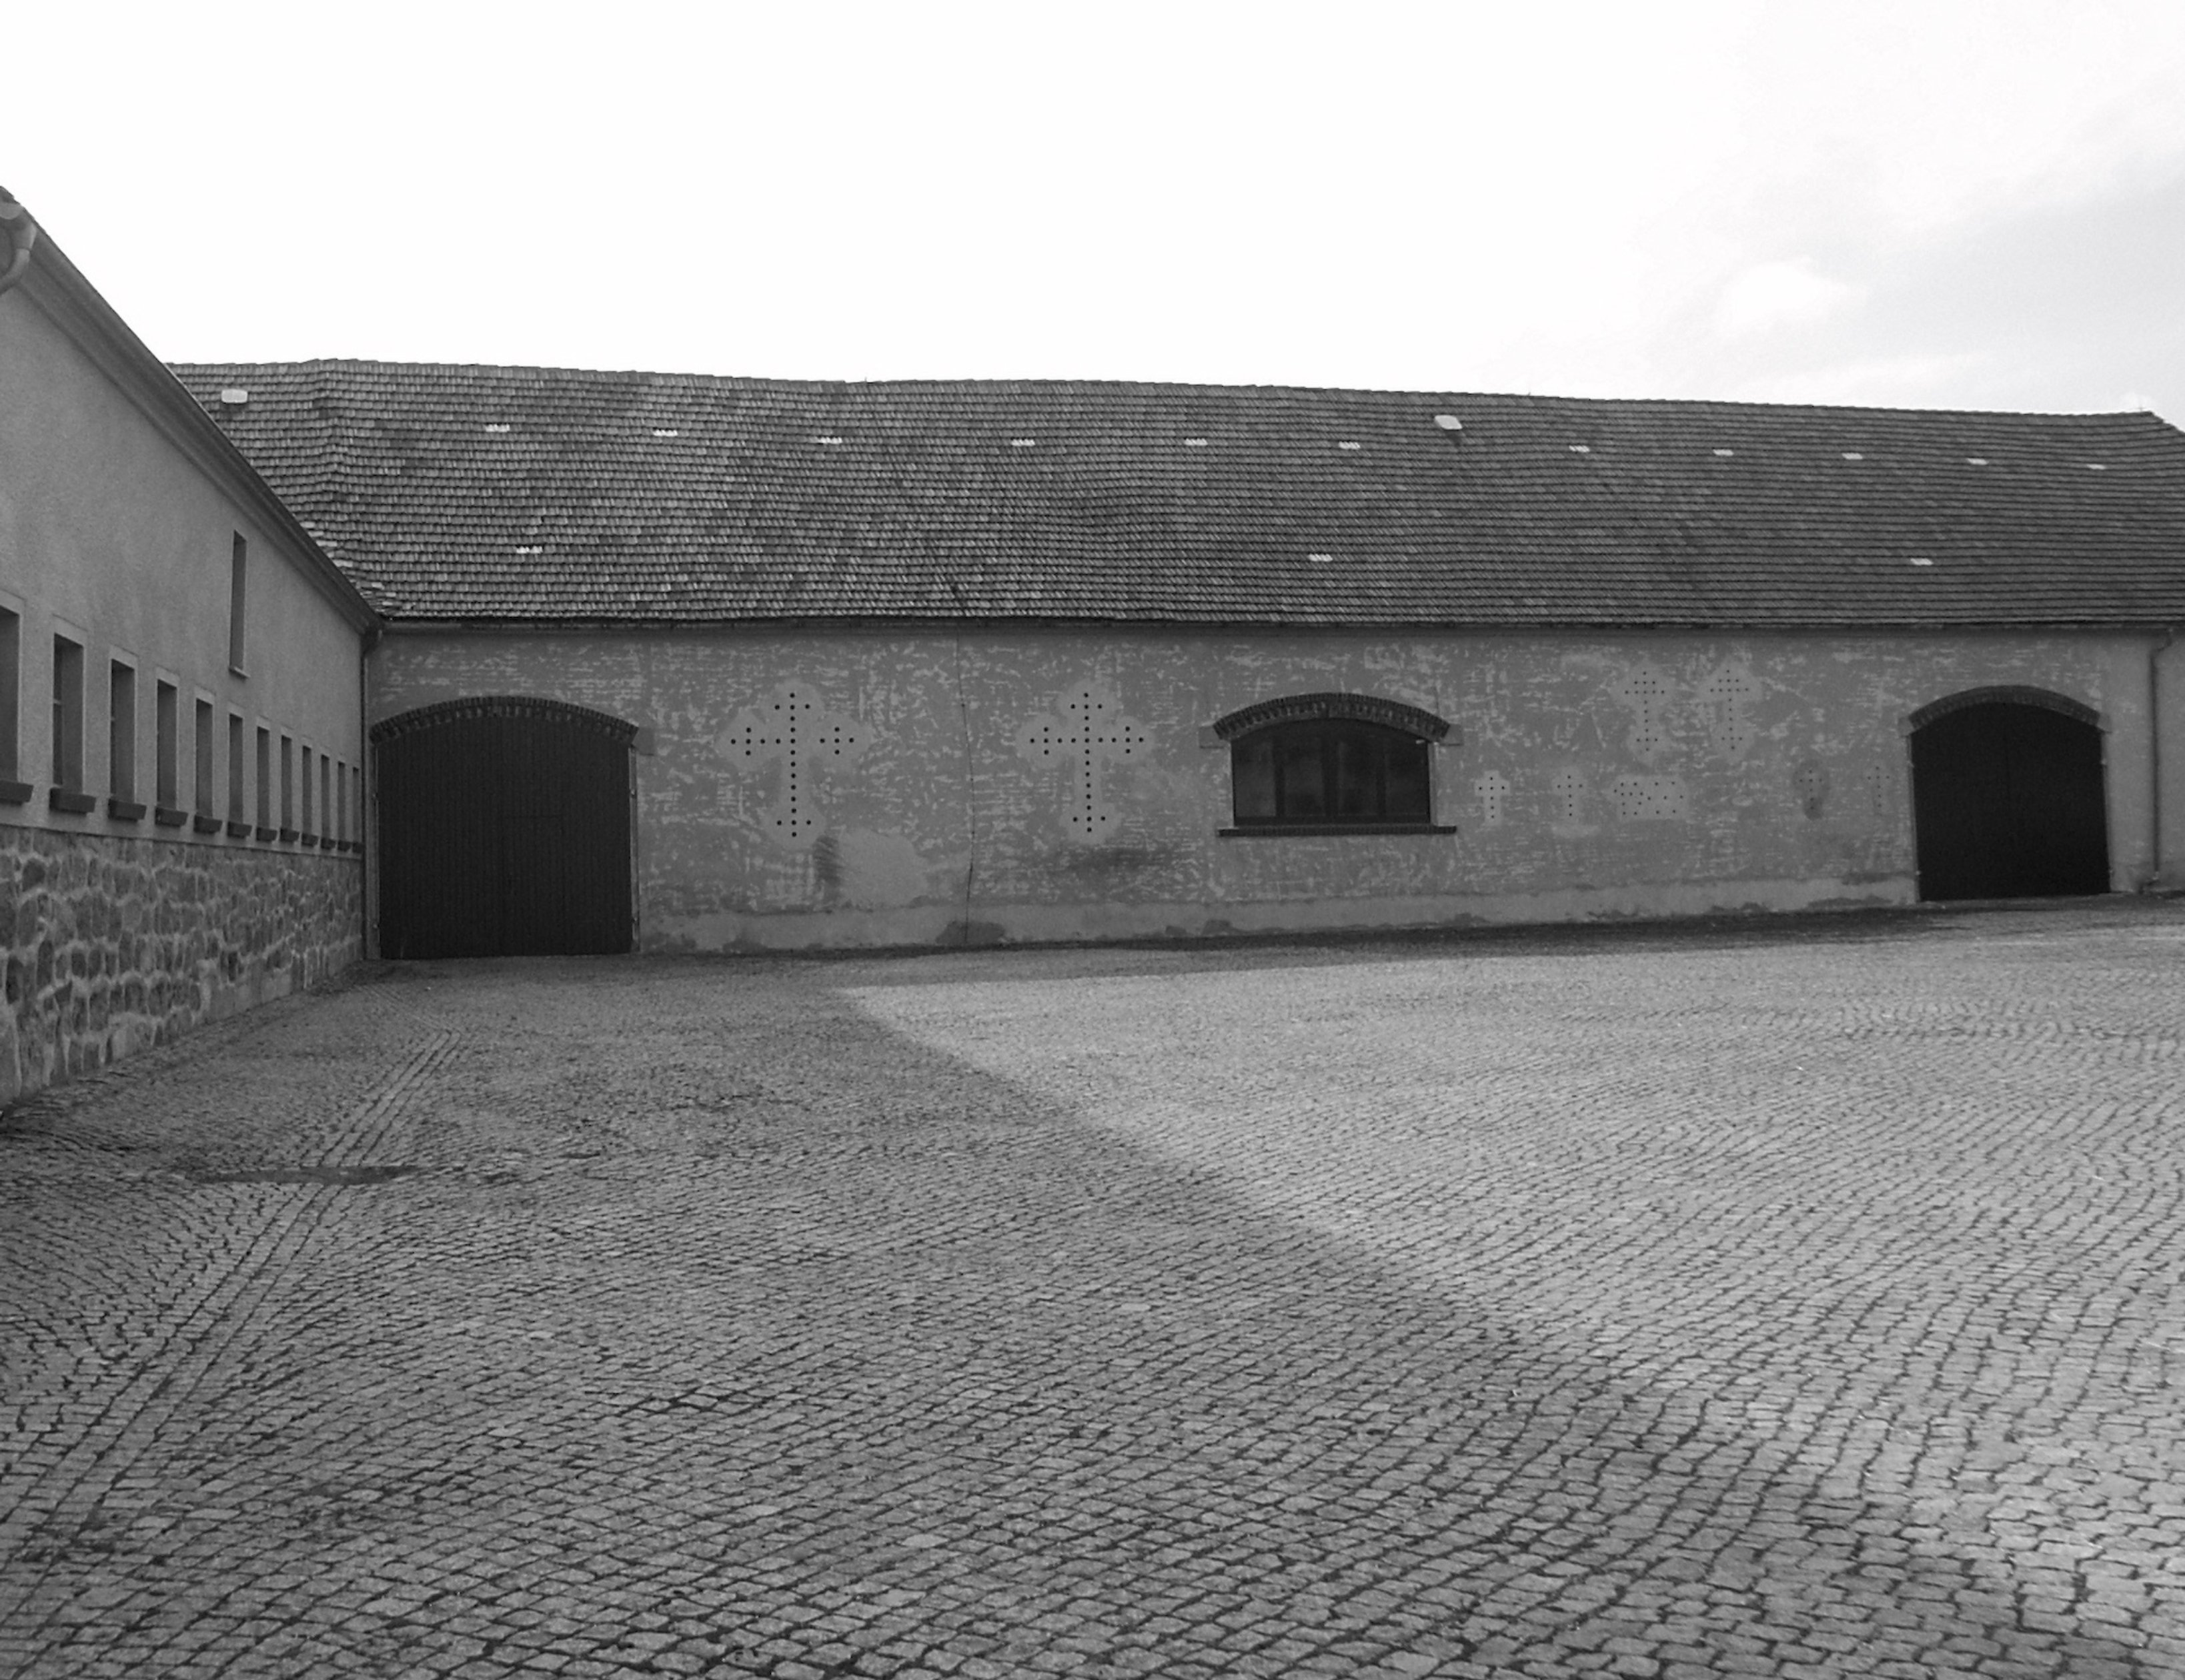
\includegraphics[width=\linewidth]{images/tm_goebel.jpg}
    \caption[Göbel's Scheune in Obersohland]{Stallung auf dem Göbelschen\protect\index{p}{Göbel} Gut in Obersohland\protect\index{o}{Obersohland}}
    \label{goebelscheune}
\end{figure}

Jakob\label{rosenbaum} Rosenbaum\index{p}{Rosenbaum, Jakob}:
\begin{leftbar}   
Vor dem Abmarsch in Obersohland\index{o}{Obersohland} fragte man beim Appell, wer von den Häftlingen nicht mehr gehen konnte. Daraufhin traten neun Leute heraus.
Vor dem Abmarsch hatte man ein Kommando von 15 Männern gewählt, die den Platz reinigen sollten, wo die Häftlinge sich aufgehalten haben. [...] Ich hatte damit gerechnet, dass, wenn wir die Arbeit beendigen werden, wird der Bauer, der Eigentümer der Scheune, uns etwas geben. Als wir die Arbeit beendet hatten, waren schon Fuhrwerke vorbereitet und die ukrainischen Posten haben befohlen, die neun Gehunfähigen auf das Fuhrwerk zu setzen. Wir haben sie aufgesetzt und außerdem zwei Tote, die vor dem Abmarsch gestorben waren. Ein Ukrainer hat dem Fuhrmann befohlen, abzufahren. Auf das zweite Fuhrwerk hat er befohlen, Schaufeln und Kreuzhacken zu legen. Wir haben sofort verstanden, was das bedeutet. Wir sind dem Fuhrwerk nachgegangen. Es war mir so finster vor Augen, dass ich kaum wusste wo ich hingehe. Auf dem ersten Fuhrwerk waren Menschen aus \L \'od\'z: mein Cousin Silberberg\index{p}{Silberberg}, an den Namen des zweiten erinnere ich mich nicht, mir scheint Rosenberg. Sein Schwager, Friede hieß er, war auch im Lager. Nach einer halben Stunde sind wir zu einem Wald gekommen. Das erste Fuhrwerk mit den Menschen war schon da. Die Ukrainer befahlen, ein Grab zu graben. Die neun Menschen, als sie das gesehen haben, sind sie in Gewein ausgebrochen. Jeder hat gebeten, dass er schon wird mit marschieren. Man soll ihm nur das Leben lassen. Mein Cousin kam zu mir mit Tränen in den Augen. 
%Die siehst Jkov von den zwei Häusern, die ich in \L \'od\'z habe, wo meine Wohnung sein wird. 
Friedes Schwager saß auf der Erde und bewegte die Lippen, die Tränen flossen ihm aus den Augen.\footnote{Jakob Rosenbaum: Von Görlitz nach Tirol, S. 39-45.}
\end{leftbar}
Janusch Oborowicz\index{p}{Oborowicz, Janusch}:
\begin{leftbar}   
Erschöpfte und kranke Häftlinge, die von Sohland\index{o}{Obersohland} aus den Marsch nicht fortsetzen konnten, jedoch andererseits mit eigenen Augen gesehen hatten, was ihren Leidensgenossen passierte, hatten sich vor dem Abmarsch in der Scheune versteckt. Der Bauer Göbel, bei dem wir untergebracht waren, hatte dies jedoch beobachtet und machte die Wachmannschaft darauf aufmerksam, worauf eine Durchsuchung der Scheune erfolgte. Die hierbei vorgefundenen Häftlinge wurden am nächsten Waldrand von der SS-Wachmannschaft erschossen.\footnote{Janusch Oborowicz. BStU MfS ASt 13/48 Bd. 2 / 393. }
\end{leftbar}

Janek Schilid\index{p}{Schilid, Janek} berichtet übereinstimmend:
\begin{leftbar}
Mit einem vom Bauer Göbel\index{p}{Göbel} zur Verfügung gestellten Fuhrwerk wurden die Häftlinge an den nächsten Waldrand gefahren, dort vom Wagen herunter geholt und von Angehörigen des Wachpersonals erschossen.\footnote{Janek Schilid, am 04.08.1914 in Jaloschin/Welonyen geboren. BStU MfS ASt 13/48 Bd. 2 / 397.}
\end{leftbar}

\newpage
%%%%%%%%%%%%%%%%
\paragraph{Lehdehäuser}
Ein Mann aus den Lehdehäuser\index{o}{Lehdehäuser}n, der nicht namentlich genannt werden möchte, sah die Häftlingskolonne am elterlichen Haus vorbeiziehen:
\begin{leftbar} 
Zusammen mit meinem kleineren Bruder beobachteten wir vorbeiziehende Häftlinge. Sie trugen längs gestreifte Kleider und eine kleine Mütze. Viele liefen barfuß, die anderen hatten sich Lumpen um die Füße gebunden. Durchweg allen konnte man ihre widrige Versorgungslage ansehen, ihre Gesichter waren eingefallen und zeugten von Unterernährung. Inmitten der Kolonne wurden mehrere großrädrige Bauernwagen, die lediglich mit Brettern belegt waren, gezogen. Ein jeder dieser zwei mal vier Meter großen Wagen wurde durch ca. 20 Häftlinge an zwei Seilen gezogen und von allen Seiten geschoben. Die Wagen waren für die Leichen sowie Grabwerkzeuge bestimmt. Der Zug wurde im Abstand von 30 Metern von SS-Wachleuten begleitet.\newline
Einige Häuser zuvor hatte Frau Talke\index{p}{Talke} einen Viertelkorb Äpfel auf die Straße geschüttet, damit sie sich die Gefangenen greifen konnten. Vor dem Haus meiner Eltern stand ein Brunnen, an dem einige Häftlinge den Schwängel betätigten, um Wasser hochzupumpen. Die SS-Wachleute ließen dies nicht zu und schlugen mit ihren Gewehrkolben auf die Dürstenden ein. Ein Häftling brach, nachdem er am Haus vorbei gelaufen war, auf der Straße zusammen. Sogleich stieß ihm ein Wachmann sein Knie in den Rücken, so dass er ganz zu Boden sank und durch einen Genickschuss getötet wurde. Ihn haben sie auf einen der Wagen geladen. Ehe alle Häftlingen an den Lehdehäuser\index{o}{Lehdehäuser}n vorbeigezogen waren, verging einige Zeit, doch viel länger dauerte es, bis das Gewehrfeuer in der Ferne verstummte.\footnote{Interview vom 16.10.2004 in den Lehdehäuser\index{o}{Lehdehäuser}n / Kemnitz.}
\end{leftbar}

Im Prozess gegen Zunker und Czech gab ein Zeuge zu Protokoll:
\begin{leftbar}   
Josef Bursztyn\index{p}{Bursztyn, Josef} war während Evakuierung so schwach geworden, dass er nicht mehr weiter gehen konnte und sich auf den Boden setzte. Zunker ging auf ihn drauf zu und forderte ihn auf, aufzustehen, worauf er Zunker bat, ihn doch zu erschießen, damit seine Qualen ein Ende haben. Zunker befahl zwei anderen Häftlingen, ihm aufzuhelfen und erschoss ihn dann.\footnote{Prozessakten von Czech. LArchB B Rep 058 Bd. 2.}
\end{leftbar}

%%%%%%%%%%%%%%%%
\paragraph{Buschschenke}
~\newline
Gerda Bötig\index{p}{Böetig, Gerda} erinnert sich heute mit Schrecken an den Todesmarsch, damals besaßen ihre Eltern die zwischen Herwigsdorf\index{o}{Buschschenke} und Kemnitz\index{o}{Kemnitz} gelegene Gastwirtschaft in der gleichnamigen Buschschenke\index{o}{Buschschenke}:
\begin{leftbar}   
Beim Eintreffen der Häftlingskolonne wollten die Gastleute den völlig ausgehungerten Gefangenen Wurstbrühe geben. Die Wachmannschaften verboten dies jedoch, und so gelang es ihnen nur, eine Wanne mit Wasser in den Hof zu stellen. Auf demselben Wege wie die Häftlingskolonne kam ich einige Zeit später aus Richtung Kemnitz\index{o}{Kemnitz} zur Buschschenke\index{o}{Buschschenke}, wo die Häftlinge bereits beim Appell standen. Etwa 100 Meter vor der Buschschenke\index{o}{Buschschenke} sah ich einen Häftling auf der Straße liegen, der vor Erschöpfung nicht mehr weiter konnte. Ich erzählte dies den SS Bewachern in der Hoffnung, dass diese dem Häftling helfen und ihn nachholen. Diese taten nicht dergleichen und entgegneten mir stattdessen: \glqq Wir machen ihn fertig\grqq.
Kurz darauf wurde der Häftling erschossen. Die Opfer zogen sie in einem Karren hinterher. Der Todesmarsch setzte sich in Richtung Strahwalde\index{o}{Strahwalde} fort.\footnote{Interview mit Gerda Bötig durch Kurt Wolf vom Sommer 2004.}
\end{leftbar}

Jakob Rosenbaum\index{p}{Rosenbaum, Jakob}: 
\begin{leftbar}   
Wir gehen weiter, wir treten auf Tote. Wir bemerken, wie im Wald ein paar Menschen sitzen. Ich schreie steht auf! Ich habe gar nicht bemerkt, dass zwei Soldaten sie bewachen und Menschen schon ein Grab graben. Als wir uns etwas entfernt haben, hörten wir eine Schießerei. Wir gehen den Weg weiter, der nach Reichenbach führt. Nach einem ganzen Tag Marschieren, sind wir in Regersdorf [gemeint ist Rennersdorf] stehen geblieben.\footnote{Jakob Rosenbaum: Von Görlitz nach Tirol, S. 39-45.}
\end{leftbar}

Am selben Weg endeckten Waldarbeiter nach dem Krieg eine mit Reisig verdeckte Grube. Unter den Zweigen lagen sieben Leichen (siehe Ermittlungen gegen die NS-Verbrechen S.~\pageref{buschschenke}).

\begin{leftbar}   
Auf dem Wege haben wir viele Tote gesehen. Ich habe unter anderem den Juden Rosensaft\index{p}{Rosensaft} aus \L \'od\'z\index{o}{Litzmannstadt} gesehen. Das Blut ist ihm aus dem Mund gerinnt. Ich habe mich ihm genähert und versucht ihn aufzustellen. Er hat mit der Hand eine Bewegung gemacht und gemeint: Rosenbojm, lass mich sterben. Ich wollte ihm erzählen, was im Wald passierte, in diesem Moment ist der Rapportführer gekommen und hat ihn erschossen.\footnote{Jakob Rosenbaum: Von Görlitz nach Tirol, S. 39-45.}
\end{leftbar}

%%%%%%%%%%%%%%%%
\paragraph{Rennersdorf}
~\newline
Am Nachmittag des 23. Februar 1945 erreichten die Häftlinge die Ortschaft Rennersdorf. 

Janusch Oborowicz\index{p}{Oborowicz, Janusch}:
\begin{leftbar}   
Nach Sohland\index{o}{Obersohland} galt als nächstes Ziel Rennersdorf, wo wir in den späten Abendstunden eintrafen. Noch wenige 100 Meter vor dem Ziel fielen einige Häftlinge vor Erschöpfung um, die dann sofort an der Straße von den Angehörigen des Wachpersonals erschossen wurden.\footnote{Janusch Oborowicz, am 25.05.1923 in Breslau geboren. BStU MfS ASt 13/48 Bd. 2 / 393.}
\end{leftbar}

Frau Liesbeth Sägner\index{p}{Sägner, Liesbeth} beobachtete im Alter von 11 Jahren die vorbeiziehenden Häftlinge:
\begin{leftbar}   
Sie waren gehüllt in Sträflingskleidung und Lumpen. Sie liefen in Zweierreihen und bildeten eine lange Kette mit vielen Unterbrechungen. Wachleute begleiteten den Zug mit ihren großen Hunden.\footnote{Liesbeth Sägner während eines Interviews in Rennersdorf, 2005.}
\end{leftbar}

Die Rennersdorferin Hildegard Fleischmann\index{p}{Fleischmann, Hildegard}:
\begin{leftbar}   
Ich befand mich seinerzeit vor der Seliger-Schmiede\index{p}{Seliger} und beobachtete, wie einer der Häftlinge vor Erschöpfung zusammenbrach. Hierauf trat ein Angehöriger des SS-Wachpersonals an den Zusammengebrochenen heran und versuchte ihn mit den Füßen in den neben der Straße fließenden Bach zu stoßen. Der Schmied Seliger\index{p}{Seliger} beobachtete gleichfalls diesen Vorfall, trat an den SS-Mann heran und sagte: \glqq Na, na, soweit ist es nicht, dass er in den Bach gekippt wird\grqq. Er bot einen Handwagen zum Abtransport des Häftlings an, womit dann der zusammengebrochene Häftling mit einem zweiten Juden, der bereits einige Zeit vorher zusammengebrochen war, weggefahren wurde.\footnote{Hildegard Fleischmann, am 02.09.1915 in Schlegel geboren. BStU MfS ASt 13/48 Bd. 2 / 460. Bestätigt wurde dies auch durch Liesbeth Sägner während eines Interviews in Rennersdorf. Auch Christa Schuberts Großmutter hat dies gesehen.}
\end{leftbar}

Die damalige Rennersdorferin Christa Schubert\index{p}{Schubert, Christa} entsinnt sich der Schrecken des 23. Februar 1945, dem Tag ihres 12. Geburtstags:

\begin{leftbar}   
Unsere Großmutter kam aus dem Oberdorf und hat sie [die Häftlinge] gesehen. Wenn sie von Berthelsdorf\index{o}{Berthelsdorf} kommen, bei der ersten Wirtschaft. Dort hat unsere Großmutter gewohnt. Und wir haben unten bei Schulzes Brücke [Abzweig Herrnhut] gewohnt und sie wollte zum Kaffee trinken zu meinem 12. Geburtstag runter kommen, da hat sie das schon von dort oben gesehen. Sie konnte sich noch erinnern, dass bei der Seliger-Schmiede, wo jetzt Bachmanns wohnen, einige nicht mehr richtig fort konnten. Dort musste der Schmied einen Leiterwagen geben. [...] Die Großmutter sah zu, dass sie weg kam. Der Zug ist dann hinterher gekommen. Das ist nach dem Mittag gewesen, denn da war ja überall Landwirtschaft, und das Vieh war zu füttern, deshalb musste in der dritten Stunde Kaffee getrunken werden. Wir haben in der Küche auf der Bank gestanden und zum Fenster raus geguckt. Ich kann mich noch genau entsinnen, weil da ein Zweiräder [Wagen] war und die Köpfe auf der Straße hingen und schleiften. Das war furchtbar. Die hatten solche großen Wagen und dort lagen Menschen drauf. Den haben die Gefangenen vorn gezogen und darauf lagen die, die nicht mehr fort konnten. Die waren furchtbar angezogen, die Sachen hingen so runter und es war ja Winter.
Mein Vater, meine Mutter auch, jeder war entsetzt; auf so etwas war ja niemand gefasst.\footnote{Interview mit Christa Schubert, Berthelsdorf, den 01.04.2005.}
\end{leftbar}
